\chapter{Test of \gls{cordic} Algortihm}\label{app:cordic_shape}
A test to validate the \gls{cordic} algorithm.

\section*{Materials and Setup}
To measure the \gls{cordic} algorithm the following materials were used:
\begin{itemize}
\item Digilent Analog Discovery 2 (Oscilloscope)
\item Digilent Waveforms 2015 (PC - software)
\item TMS320C5515 eZdsp development board
\end{itemize}

The materials were set up as in \autoref{chap:effect_test_response} \autoref{fig:appendix:dsp_frequency_response}, where only Ch2 is measured and $V_s$ is grounded.

\section*{Test Procedure}
The following steps were made to test the \gls{cordic} algorithm.
\begin{itemize}
\item The \gls{cordic} algorithm program, attached in the Zip-file, "cordic_2.asm", is set to make a \SI{0.5}{\hertz} sine wave.
\item The $\cos(\theta)$ and $\sin(\theta)$ is changed until the signal i stable.
\item If an offset is observed on the signal, this is removed by subtracting an iteratively found value from the signal.
\end{itemize} 

\section*{Results} 

\begin{figure}[htbp!]
	\centering
		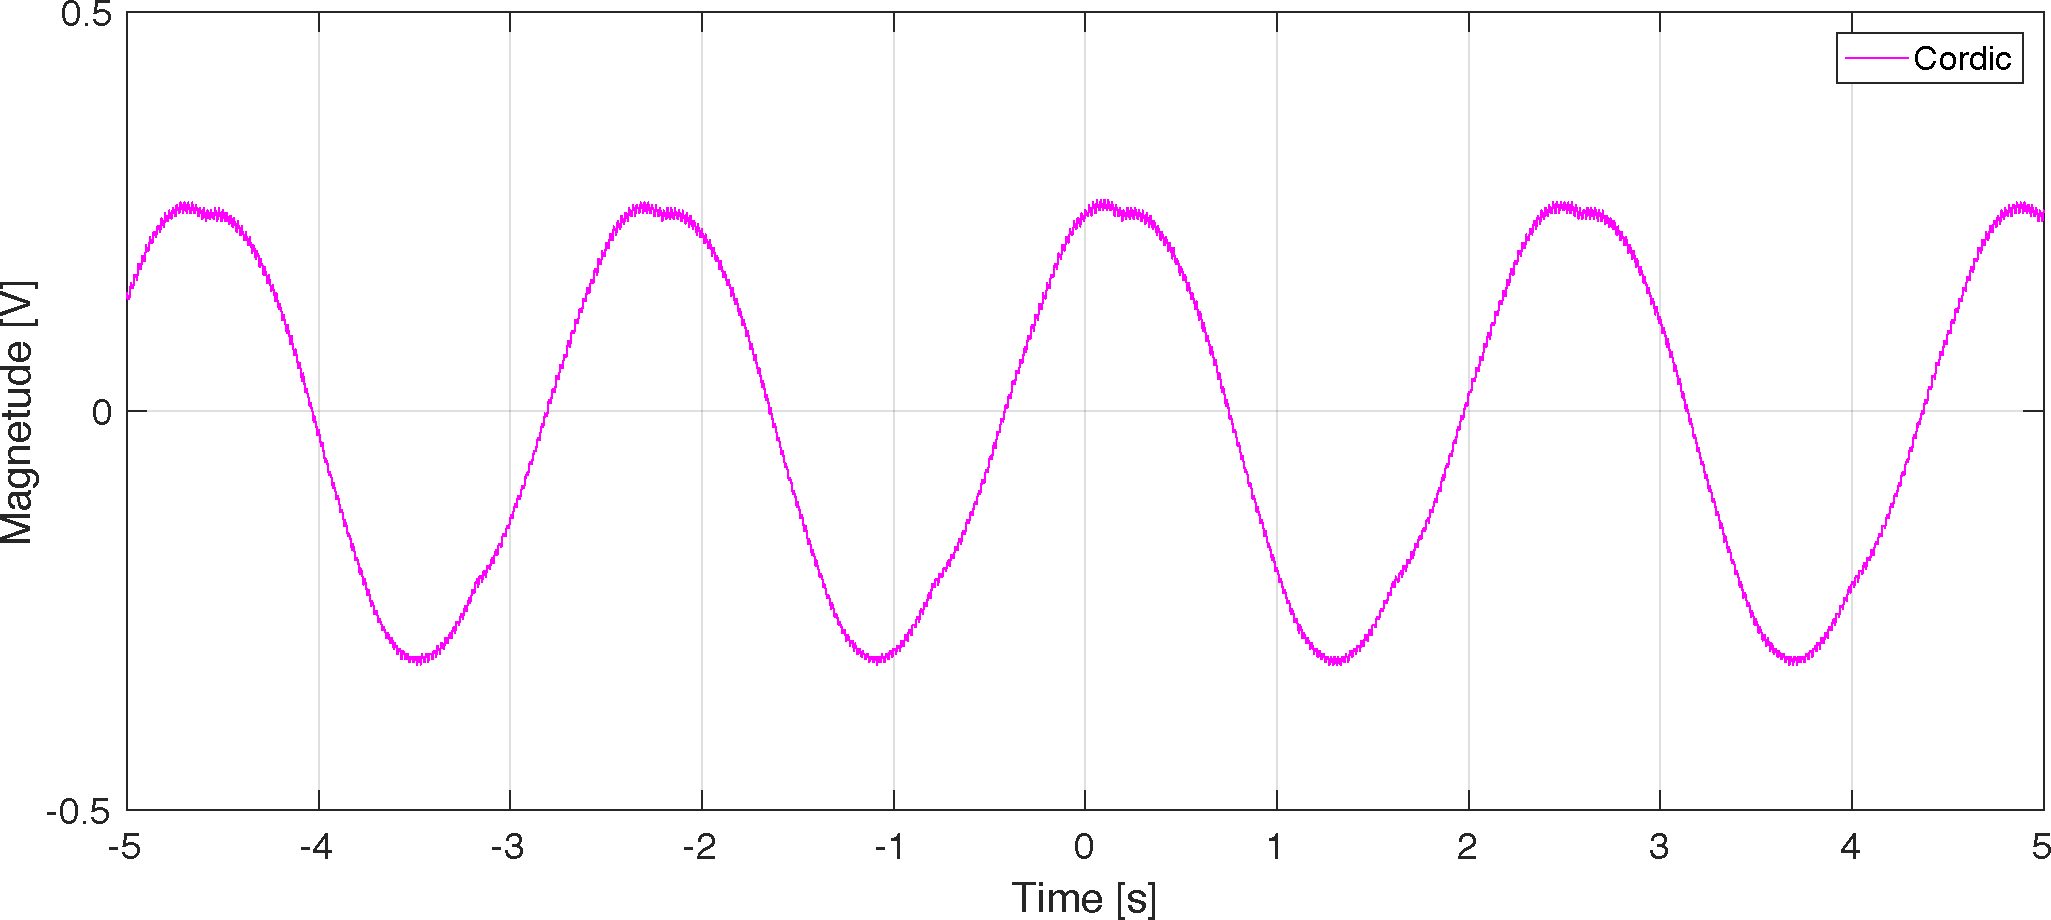
\includegraphics[width=1\textwidth]{cordic_435mHz.pdf}
		\caption{Measured signal from the \gls{cordic} algorithm, when set to produce a \SI{0.5}{\hertz} sine.}
		\label{fig:appendix:cordic_435mHz}
\end{figure}

The signal in \autoref{fig:appendix:cordic_435mHz} is measured to have a frequency of \SI{0.435}{\hertz}.